 \chapter{Metodologia de pesquisa}

Segundo \citeonline[pág.~2]{rodrigues2007}, a pesquisa deve conter um conjunto de abordagens, técnicas e processos para formular e resolver problemas do mundo real de maneira organizada e sistemática.

Para que uma pesquisa fique bem estruturada é necessário responder como os objetivos serão alcançados e  como será realizada a resolução do problema de pesquisa. Para isso, deve-se classificar a pesquisa, identificar as atividades e estabelecer como as atividades serão executadas \cite{forcon2014}.

\section{Classificação da Pesquisa}

Segundo \citeonline[pág.~41]{gil2008}, a metodologia de pesquisa é classificada através de critérios bem definidos com base em seus objetivos e procedimentos técnicos.

É usual classificar uma pesquisa com base em seus objetivos em três grandes grupos: exploratórias, descritivas e explicativas. Já em nível de procedimento técnico, a pesquisa pode ser classificada como estudo de caso, pesquisa ação, survey, experimental, entre outras \citeonline[pág.~41]{gil2008}.

A pesquisa exploratória é utilizada pelo pesquisador para familiarizar com um assunto pouco explorado. Ao decorrer ou no final da pesquisa exploratória, o pesquisador poderá estar apto para formular hipóteses \cite{giudice}.

A pesquisa descritiva é usada quando se tem um conhecimento do assunto e se quer descrever um fenômeno. Hipóteses podem ser formuladas com base em conhecimentos prévios, procurando confirmá-las ou negá-las \cite[pág.~21]{fonseca2002}.

A pesquisa é classificada com base em procedimentos técnicos em quantitativa e qualitativa. A pesquisa quantitativa traduz em números os estudos realizados e se utiliza técnicas estatísticas para comprovar os fatos \cite[pág.~9]{rodrigues2007}


As pesquisas atuais revelam que o reconhecimento mútuo e integração das abordagens qualitativas e quantitativas já é reconhecido \cite{serapioni}.

O estudo de caso é um estudo profundo, recomendável para temas muito complexos, em que é muito dificil gerar generalizações \cite[pág.~33]{fonseca2002}.

O estudo de caso vem sendo utilizado tanto em pesquisas exploratórias quanto descritivas e explicativas. É de sua natureza adotar na maioria dos casos, uma abordagem qualitativa, mas nada impede que o estudo de caso trabalhe com abordagens quantitativas \cite[pág.~22]{yin}.

Considerando os objetivos de estudo deste trabalho, foi incorporada uma pesquisa exploratória com o intuito de evidenciar os possíveis fenômenos que se repetem no mercado de moedas e uma pesquisa descritiva para evidenciar os benefícios da abordagem multiparadigma do software InvestMVC e da qualidade de código tanto a nível de testes unitários quanto a nível de análise estática de código.

Em relação aos procedimentos técnicos, foi utilizado o estudo de caso, pois apesar deste trabalho ter uma abordagem quantitativa dos dados e envolvimento de métodos matemáticos para elaboração de estratégias, não é possível afirmar que os resultados podem ser generalizados para outros contextos, como por exemplo, para a bolsa de valores ou até mesmo um par de moedas diferente do euro-dólar.

\section{Atividades da Pesquisa}

É necessário evidenciar na metodologia de pesquisa quando começam as atividades e quais são as coordenadas para que as mesmas sejam cumpridas \cite{forcon2014}.

A Figura \ref{metodologia} evidencia como estão organizadas as atividades deste trabalho.

\begin{figure}[H]
\centering
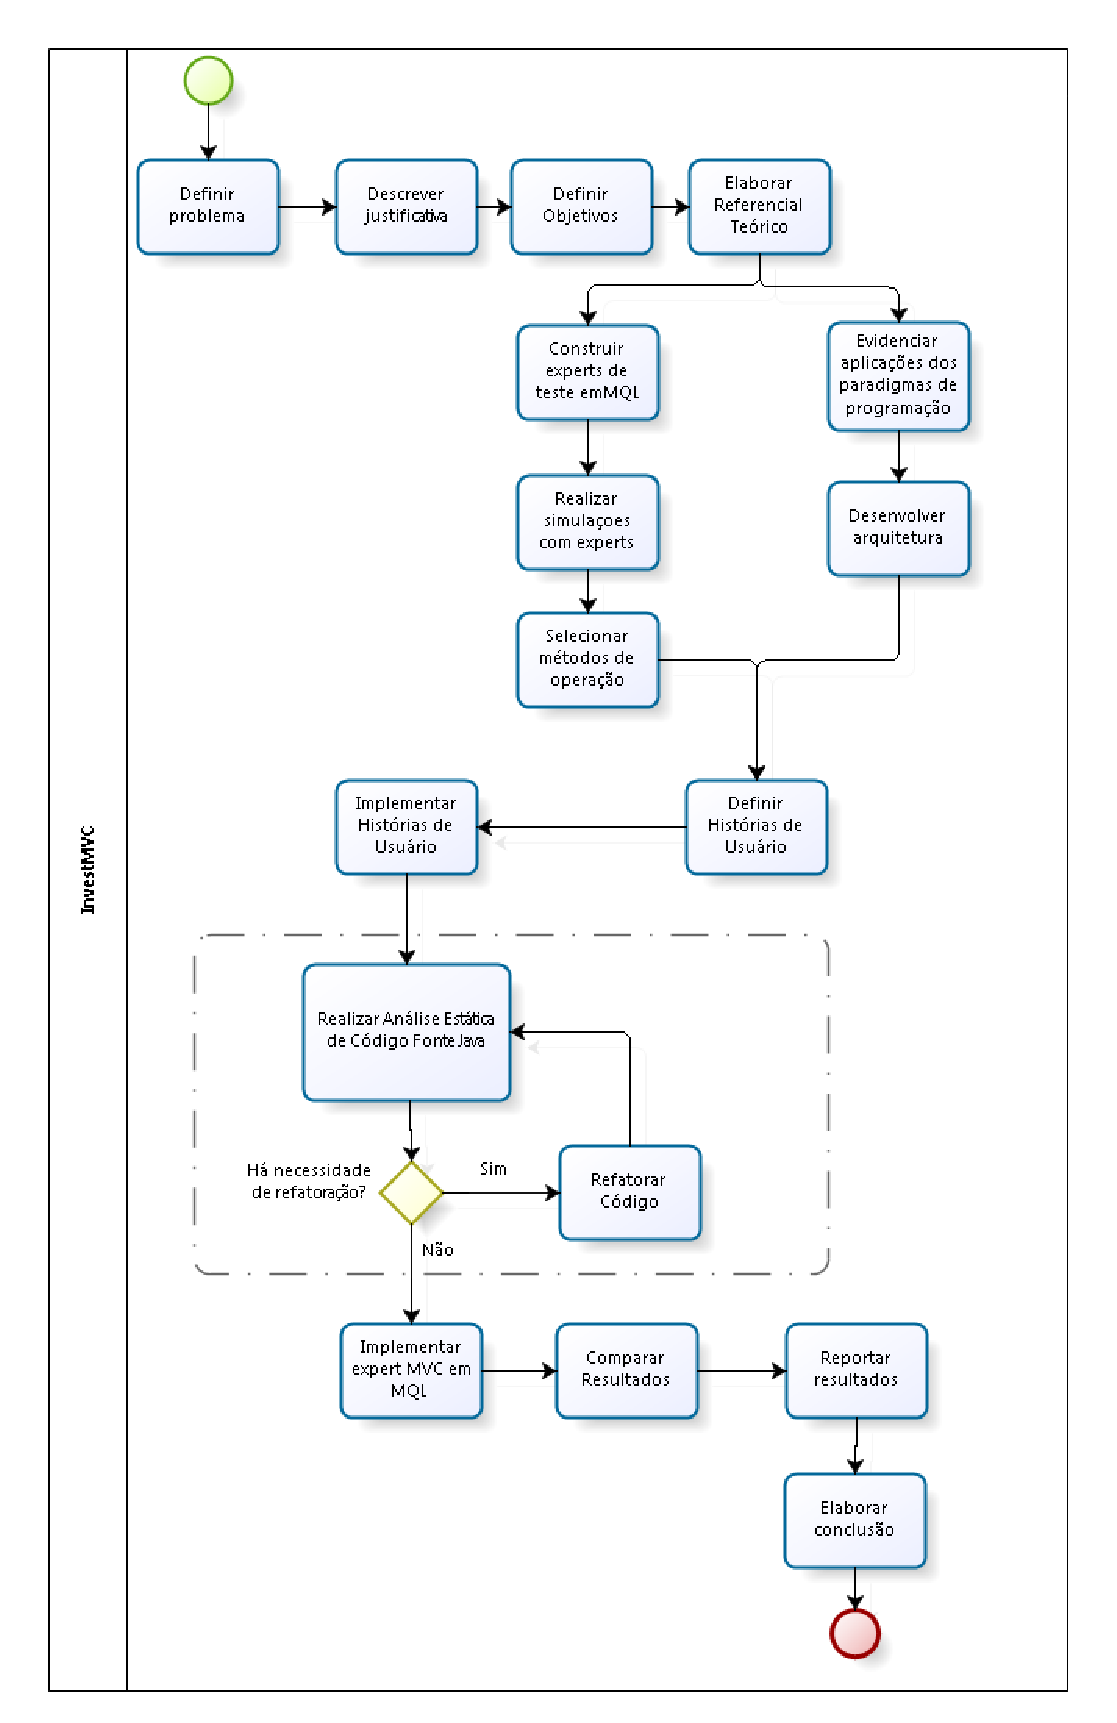
\includegraphics[width=0.7\textwidth]{figuras/metodologiaTCC}
\caption{Atividades da Pesquisa.} 
\label{metodologia}
\end{figure}

\subsection{Descrição dos Objetivos das Atividades de Pesquisa}

A Tabela \ref{atividadeMetologia}  evidencia cada atividade da pesquisa e o objetivo de cada atividade.

\begin{center}
\begin{longtable}{| p{8cm} | p{8cm} |}
\caption{Atividades e objetivos da pesquisa} \\
\hline
\textbf{Atividade} & \textbf{Objetivo} \\ \hline
\endfirsthead
\multicolumn{2}{c}%
{\tablename\ \thetable\ -- \textit{Continuação da página anterior}} \\
\hline
\textbf{Atividade} & \textbf{Objetivo} \\ \hline
\endhead
\hline \multicolumn{2}{c}{\textit{Continuação na próxima página}} \\
\endfoot
\hline
\endlastfoot
	Definir problema & Definir o problema de pesquisa do trabalho.\\ \hline
	Descrever justificativa & Com base no problema de pesquisa, deve-se justificar a relevância do trabalho proposto.\\ \hline
	Elaborar referencial teórico & Com base na literatura, descrever os conceitos chaves como Contexto Financeiro, Paradigmas de Programação e Qualidade de Software.\\ \hline
	Construir \textit{experts} em mql & Implementar \textit{expert} Fibonacci.mql, MinimosQuadrados.mql, CorrelacaoLinear.mql, Estocastico.mql, MediaMovel.mql. \\ \hline
	Realizar simulação com \textit{experts} & Definir critérios de entrada e saída para cada \textit{expert} e realizar a simulação de cada \textit{expert} no Mercado de Moedas durante o perído de 2 anos (agosto 2012-2014).\\ \hline
	Selecionar métodos de operação & Selecionar os métodos (Fibonacci, Mínimos Quadrados, Correlação Linear, Estocástico ou Média Móvel) que obtiverem lucro durante o período de simulação.\\ \hline
	Evidenciar aplicações paradigmas de programação & Evidenciar aplicações dos paradigmas: funcional, lógico, estruturado e multiagente.\\ \hline
	Desenvolver arquitetura & Desenvolver a arquitetura da ferramenta InvestMVC no intuito de evidenciar decisões sobre a organização do sistema.\\ \hline
	Definir Histórias de Usuário & Definir o conjunto de funcionalidades e pontuar cada História, seguindo a sequência de Fibonacci para realizar a pontuação.\\ \hline
	Implementar Histórias de Usuário & Desenvolver as Histórias de Usuário que foram definidas.\\ \hline
	Realizar Análise Estática de Código Fonte & Realizar a análise estática de código fonte para aferir o nível de qualidade do código fonte da ferramenta InvestMVC.\\ \hline
	Implementar \textit{expert} em MQL & Implementar toda a lógica da ferramenta InvestMVC em linguagem MQL.\\ \hline
	Comparar resultados monetários \textit{expert} MQL e ferramenta InvestMVC & Comparar os resultados monetários do \textit{expert} em mql com a ferramenta InvestMVC durante um tempo a se determinado de operação.\\ \hline
	Reportar resultados & Registrar os resultados da comparação do desempenho da ferramenta InvestMVC e do \textit{expert} em MQL.\\ \hline
	Elaborar conclusões & Desenvolver as conclusões do trabalho.\\
\label{atividadeMetologia}
\end{longtable}
\end{center}

\section{Execução da Pesquisa}

Scrum é uma metodologia de desenvolvimento fundada na teoria do controle de processos empíricos. O empirismo afirma que conhecimento vem da experiência. As decisões são tomadas com base na experiência em que se tem de um determinado assunto. Scrum emprega uma abordagem iterativa e incremental para otimizar a previsibilidade e controle de riscos da execução de um projeto. Existem três pilares que sustentam qualquer implementação de controle de processos empíricos: transparência, inspeção e adaptação \cite[pág.~4]{schwaber2013}.

Neste trabalho, vertentes defendidas pelo Scrum foram adaptadas e incorporadas à metodologia de pesquisa. Os produtos de  trabalho foram alocados e desenvolvidos em Sprints (intervalo de tempo de 1 a 4 semanas). Durante a execução de cada Sprint, foram realizadas as adaptações necessários para que os produtos de trabalho fossem produzidos com sucesso.

Na Sprint 1, foi construída a proposta de trabalho e foi implementado os métodos matemáticos em linguagem C que serviram como prova de conceito para viabilizar o desenvolvimento do trabalho.

Na Sprint 2, foi construído o referencial teórico dos métodos matemáticos e paradigmas de programação. Também foi feito um protótipo da ferramenta InvestMVC para evidenciar como seria a \textit{view} da ferramenta com a dinâmica de construir um robô, selecionar e ativar um robô.

Na Sprint 3, foram refinados o referencial teórico feito na Sprint 2 e foi construído o referencial teórico do Contexto Financeiro.

Na Sprint 4, foi definida a metodologia de pesquisa e foram descritas algumas aplicações dos paradigmas de programação.

A Sprint 5 foi utilizada para atender os resultados do primeiro objetivo específico do trabalho (i.e. selecionar os métodos matemáticos do software InvestMVC). Para isso, foram utilizadas simulações para os métodos de fibonacci, correlação de Pearson, mínimos quadrados, média móvel e estocástico. Para realizar essas simulações, foram construídos \textit{experts} para cada método matemático. Ao final das simulações, foram selecionados os métodos matemáticos de correlação de Pearson, fibonacci e mínimos quadrados.

A Sprint 6 foi utilizada para definir o backlog de Histórias de Usuário. As pontuações de cada História foram definidas com base na complexidade de cada uma. Nessa Sprint, também foi realizada a análise estática de código fonte do paradigma estruturado e obteve-se uma qualidade de código aceitável.

Na Sprint 7, foi definido que seriam desenvolvido as Histórias de Usuário US1 (Agente Correlação Linear), US5 (Agente gestor), US11(ativar Expert) e US12 (desativar Expert). Não foi possível terminar, as Histórias US11 e US12 nessa Sprint.

Na Sprint 8, foram desenvolvidas as Histórias US11 e US12 que não haviam sido terminadas na Sprint anterior. Foram desenvolvidas as Histórias de Usuário US4 (Agente Tendência), US2 (Agente Fibonacci) e US17 (método Fibonacci em linguagem Haskell). Com essas Histórias de Usuários implementadas, já foi possível disponibilizar a primeira versão do software InvestMVC.

A Sprint 9 estava prevista para construir a US18 (método de Mínimos Quadrados em linguagem Haskell) e US7 (acompanhar retorno financeiro). Entretanto, foi refeito o planejamento dessa Sprint para atender demandas com maior prioridade. A Sprint 9 foi destinada para realizar alguns ajustes metodológicos e escrever os resultados obtidos com as Histórias de Usuário desenvolvidas nas Sprints anteriores. Além disso, foi elaborado um formulário para obter o \textit{feedback} dos usuários que começaram a utilizar a primeira versão da ferramenta na Sprint anterior. Infelizmente, foi detectado que os resultados obtidos na execução dos códigos feitos em linguagem C e em linguagem Haskell não forneciam resultados similares. Como consequência nem todos os resultados previstos foram documentados nessa Sprint.

Devido aos acontecimentos ocorridos na Sprint 9, a Sprint 10 foi totalmente replanejada, criando uma nova Sprint para alocar as atividades que eram da Sprint 10.

Na Sprint 10, foi detectada a necessidade de excluir a US20 (retirar da base de conhecimento). Foi realizada a análise estática de código fonte dos paradigmas multiagente e estruturado. Os resultados da qualidade de código e os resultados não documentados da Sprint anterior foram feitos.

Na Sprint 11, foi construída a US22 (Expert no componente MQL), permitindo a integração entre o componente MQL e Multiagente \textit{expert}. Sendo assim, uma versão estável da ferramenta InvestMVC ficou pronta.

\section{Cronograma}

A Tabela \ref{cronograma} mostra quais foram as atividades em cada Sprint e a duração da mesma. O cronograma detalhado encontra-se no apêndice A - Cronograma InvestMVC.

\begin{center}
\begin{longtable}{  | p{2cm} | p{8cm} | p{2cm}| p{2cm} |}
\caption{Cronograma simplificado} \\
\hline
\textbf{Sprint} & \textbf{Atividades} & \textbf{Data de início} & \textbf{Data de finalização}\\ \hline
\endfirsthead
\multicolumn{4}{c}%
{\tablename\ \thetable\ -- \textit{Continuação da página anterior}} \\
\hline
\textbf{Sprint} & \textbf{Atividades} & \textbf{Data de início} & \textbf{Data de finalização} \\ \hline
\endhead
\hline \multicolumn{4}{c}{\textit{Continuação na próxima página}} \\
\endfoot
\hline
\endlastfoot
    
    Sprint 1 & \begin{enumerate}
    \item Construir introdução
    \item Implementar Métodos Numéricos
    \end{enumerate} & 10/08/2014 & 31/08/2014\\ \hline
    
    Sprint 2 & \begin{enumerate}
    \item Construir Referencial Teórico Paradigmas de Programação
    \item Adaptar Métodos Numéricos
    \item Prototipar View Projeto
    \item Construir Referencial Teórico Métodos Numéricos
    \end{enumerate} & 01/09/2014 & 15/09/2014\\ \hline
    
    Sprint 3 & \begin{enumerate}
    \item Refinar Referencial Teórico Paradigmas
    \item Construir Referencial Teórico de Contexto Financeiro
    \item Revisar Referencial Teórico Métodos Numéricos
    \end{enumerate} & 16/09/2014 & 30/09/2014\\ \hline
    
    Sprint 4 & \begin{enumerate}
    \item Realizar Experimentos Métodos de Operação
    \item Revisar Referencial Teórico Contexto Financeiro
    \item Desenvolver Experts em MQL4
    \end{enumerate} & 01/10/2014 & 15/10/2014\\ \hline
    
    Sprint 5 & \begin{enumerate}
    \item Descrever Metodologia de Pesquisa
    \item Realizar Experimentos Métodos de Operação
    \item Evidenciar Aplicações Paradigmas de Programação
    \end{enumerate} & 16/10/2014 & 31/10/2014\\ \hline
    
    Sprint 6 & \begin{enumerate}
    \item Definir Backlog de Histórias de Usuário
    \item Verificar Qualidade de código fonte
    \end{enumerate} & 01/11/2014 & 10/11/2014\\
\label{cronograma}
\end{longtable}
\end{center}

\section{Planejamento para seleção dos métodos matemáticos}

Esta seção descreve o planejamento para seleção dos métodos matemáticos para operar de forma automatizada no mercado de moedas. O planejamento da seleção é uma adaptação do protocolo presente no Anexo A \cite{brereton}.

\subsection{Projeto para seleção dos métodos matemáticos}

Para se selecionar os métodos de operação no Mercado de Moedas da ferramenta investMVC, foi definido as seguintes variáveis e seus devidos valores:

\begin{itemize}
\item Alavancagem com valor de 0.25;
\item Conta de simulação com valor inicial de 3.000 USD;
\item Margem de negociação/alavancagem da conta igual a 1:500;
\item Stop loss e take profit definido em 500 pontos.
\item Experts programados em linguagem MQL4
\item Simulação realizada no mesmo período de tempo (agosto de 2012 à agosto de 2014)
\item Simulações realizadas na mesma máquina e mesmo sistema operacional
\end{itemize}

\subsection{Critério para seleção dos métodos matemáticos}

Os Métodos Matemáticos implementados em linguagem MQL4 que obteram lucro de 10\% do capital inicial foram aprovados no experimento.

\subsection{Definições para simulação dos métodos de operação}

Foi utilizado o simulador da plataforma Metatrader para realizar a simulação e, posteriormente, analisar os resultados e definir os métodos a serem implementados na ferramenta InvestMVC.

\subsection{Limitações da seleção dos métodos matemáticos}

A linguagem MQL4 não possui suporte para teste unitário. Portanto, os experts programados para este estudo de caso, não possuem testes automatizados.

O simulador do MetaTrader possui código fonte fechado. Portanto, não foi possível realizar adaptações do simulador através do código fonte.


\section{Planejamento para comparação dos valores monetários}

Esta seção descreve o planejamento para comparação dos resultados monetários da ferramenta InvestMVC com o expert tradicional implementado em linguagem MQL. O planejamento da seleção é uma adaptação do protocolo presente no Anexo B \cite{brereton}.

\subsection{Projeto para comparação dos valores monetários}

Para realizar a comparação dos valores monetários do software InvestMVC com o software tradicional em linguagem MQL, foram definidas variáveis de operação iguais para ambos os produtos de software:

\begin{itemize}
\item Alavancagem com valor de 0.1
\item Conta de simulação com valor inicial de 5.000 USD
\item Margem de negociação/alavancagem da conta igual a 1:500
\item Stop loss e take profit definidos de acordo com a estratégia do método de mínimos Quadrados
\end{itemize}

\subsection{Definições para execução dos produtos de software}
O software InvestMVC e o software implementado na linguagem MQL irão rodar no sistema operacional Linux.